\documentclass[tikz,border=7pt]{standalone}
\usepackage[T1]{fontenc}
\usepackage{lmodern}
\usetikzlibrary{arrows.meta,positioning,shapes.geometric,fit,backgrounds,calc}
\begin{document}
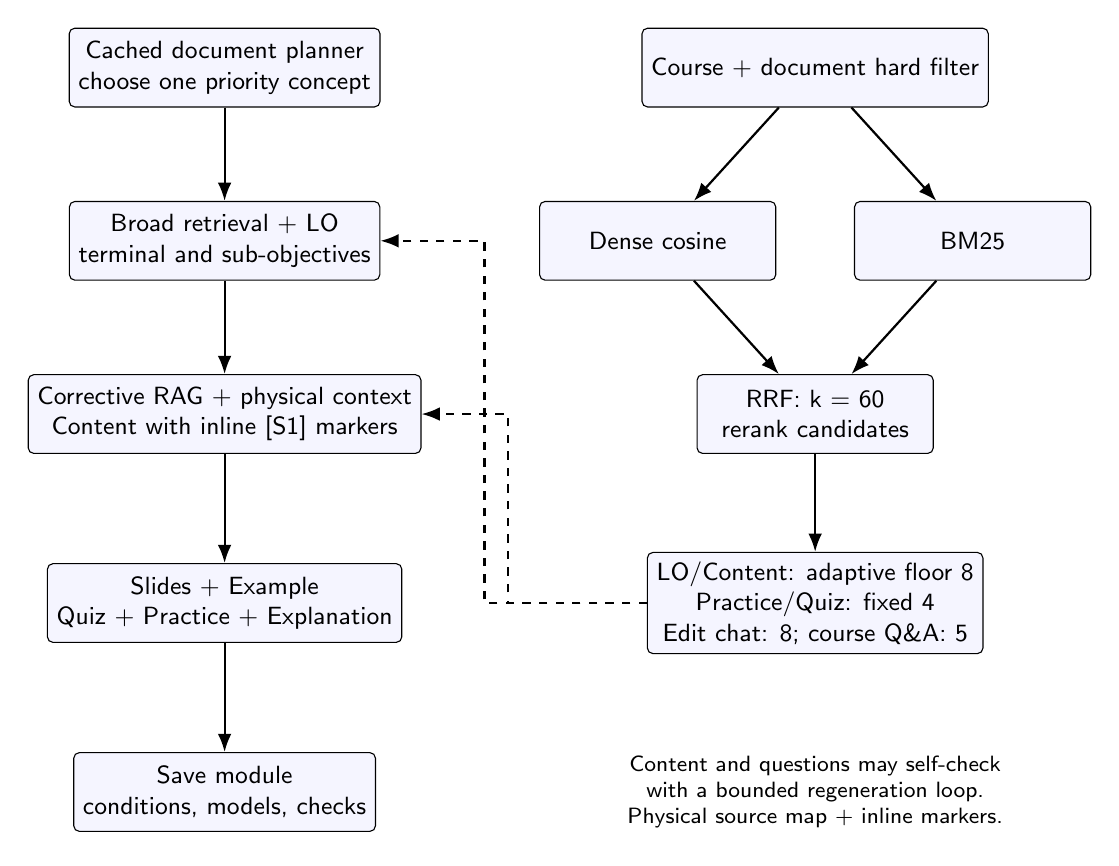
\begin{tikzpicture}[font=\sffamily\small,>=Latex,
box/.style={draw,rounded corners=2pt,align=center,minimum width=3cm,minimum height=1cm,fill=blue!4},
entity/.style={draw,rectangle,align=center,minimum width=2.6cm,minimum height=.75cm,fill=blue!4},
rel/.style={draw,diamond,aspect=2,inner sep=2pt,align=center,font=\sffamily\footnotesize,fill=yellow!8},
attr/.style={draw,ellipse,inner sep=3pt,font=\sffamily\footnotesize},
uc/.style={draw,ellipse,align=center,minimum width=4cm,minimum height=.9cm},
flow/.style={->,thick},lab/.style={font=\sffamily\scriptsize,fill=white,inner sep=2pt}]

\node[box] (planner) at (0,8) {Cached document planner\\choose one priority concept};
\node[box] (lo) at (0,5.8) {Broad retrieval + LO\\terminal and sub-objectives};
\node[box] (content) at (0,3.6) {Corrective RAG + physical context\\Content with inline [S1] markers};
\node[box] (other) at (0,1.2) {Slides + Example\\Quiz + Practice + Explanation};
\node[box] (save) at (0,-1.2) {Save module\\conditions, models, checks};
\draw[flow] (planner) -- (lo); \draw[flow] (lo) -- (content);
\draw[flow] (content) -- (other); \draw[flow] (other) -- (save);
\node[box] (scope) at (7.5,8) {Course + document hard filter};
\node[box] (dense) at (5.5,5.8) {Dense cosine};
\node[box] (sparse) at (9.5,5.8) {BM25};
\node[box] (rrf) at (7.5,3.6) {RRF: k = 60\\rerank candidates};
\node[box] (k) at (7.5,1.2) {LO/Content: adaptive floor 8\\Practice/Quiz: fixed 4\\Edit chat: 8; course Q\&A: 5};
\draw[flow] (scope) -- (dense); \draw[flow] (scope) -- (sparse);
\draw[flow] (dense) -- (rrf); \draw[flow] (sparse) -- (rrf); \draw[flow] (rrf) -- (k);
\draw[flow,dashed] (k.west) -- (3.3,1.2) |- (lo.east);
\draw[flow,dashed] (k.west) -- (3.6,1.2) |- (content.east);
\node[align=center,font=\sffamily\footnotesize] at (7.5,-1.2) {Content and questions may self-check\\with a bounded regeneration loop.\\Physical source map + inline markers.};
\end{tikzpicture}
\end{document}
